\infolevone{
\subsection{The Wire Chamber Gas Mixing System}
\label{sec:chambergas}
% (BDS) Largely pulled from detailed gas_system_HOWTO document
}
\infoleveqnull{
\section{Detector Gas Supply System}
}

The Hall~C wire chamber gas mixing system is located in the gas shed located
to the left of the counting house (when facing the counting house)
in the parking lot between the counting house
and the accelerator service building (building 96C).  The SHMS gas sysystem for
the SHMS Noble Gas Cherenkov is also located in this shed.
The gas cylinders in use are along the outside of the Gas Shed
in a fenced area. There are racks next to the Gas Shed for storage
of full gas cylinders.  Hall C currently uses ethane, argon, ethanol,
carbon dioxide, nitrogen and neon.
\infolevone{

The main
component of the system is a single MKS 647 menu driven 4-channel
controller that maintains the mix proportions and pressure regulation of the
gas supplied to the wire chambers.  Gas flow is
controlled by 2259c proportional mass flow control valves.  The 647 allows
the Gas Calibration factor to be altered in software, allowing the user to
change to a different gas without recalibration of the mass flow control
valves.

A temperature controlled alcohol bubbler is provided for the gas
stream.  The alcohol level in the stream is maintained by a float valve
fed from a reservoir outside the bubbler chiller. This allows the alcohol
system to be refilled without opening the system to air.  A sight glass on
the side of the reservoir allows the level to be monitored.  A bypass loop
around the alcohol system is provided should alcohol-free gas be desired,
or if the alcohol system requires maintenance.  Remote monitoring and limited
controls are provided through an EPICS display screen accessible via
\textbf{JMenu/Monticello $\rightarrow$ Hall C $\rightarrow$ Hall C Gas Shed},
or equivalent\footnote{Path to EDM file is /cs/opshome/edm/hlc/HLC\_gas\_shed.edl}.

{\bf This system operates by measuring and controlling pressure, not flow rate.
This system will work to maintain a pressure, regardless of the flow rate.
This allows the (pressure dependent) Rotameter-style flow meters to provide
a constant flow rate to detector systems.  Nevertheless, it should not be used
without appropriate pressure relief device such as relief bubblers and relief
valves.}

The manual valves used in this system are numbered on their
handles.  Those numbers are referenced in this document and in
Figure~\ref{fig:gas_mix}.
\begin{figure}
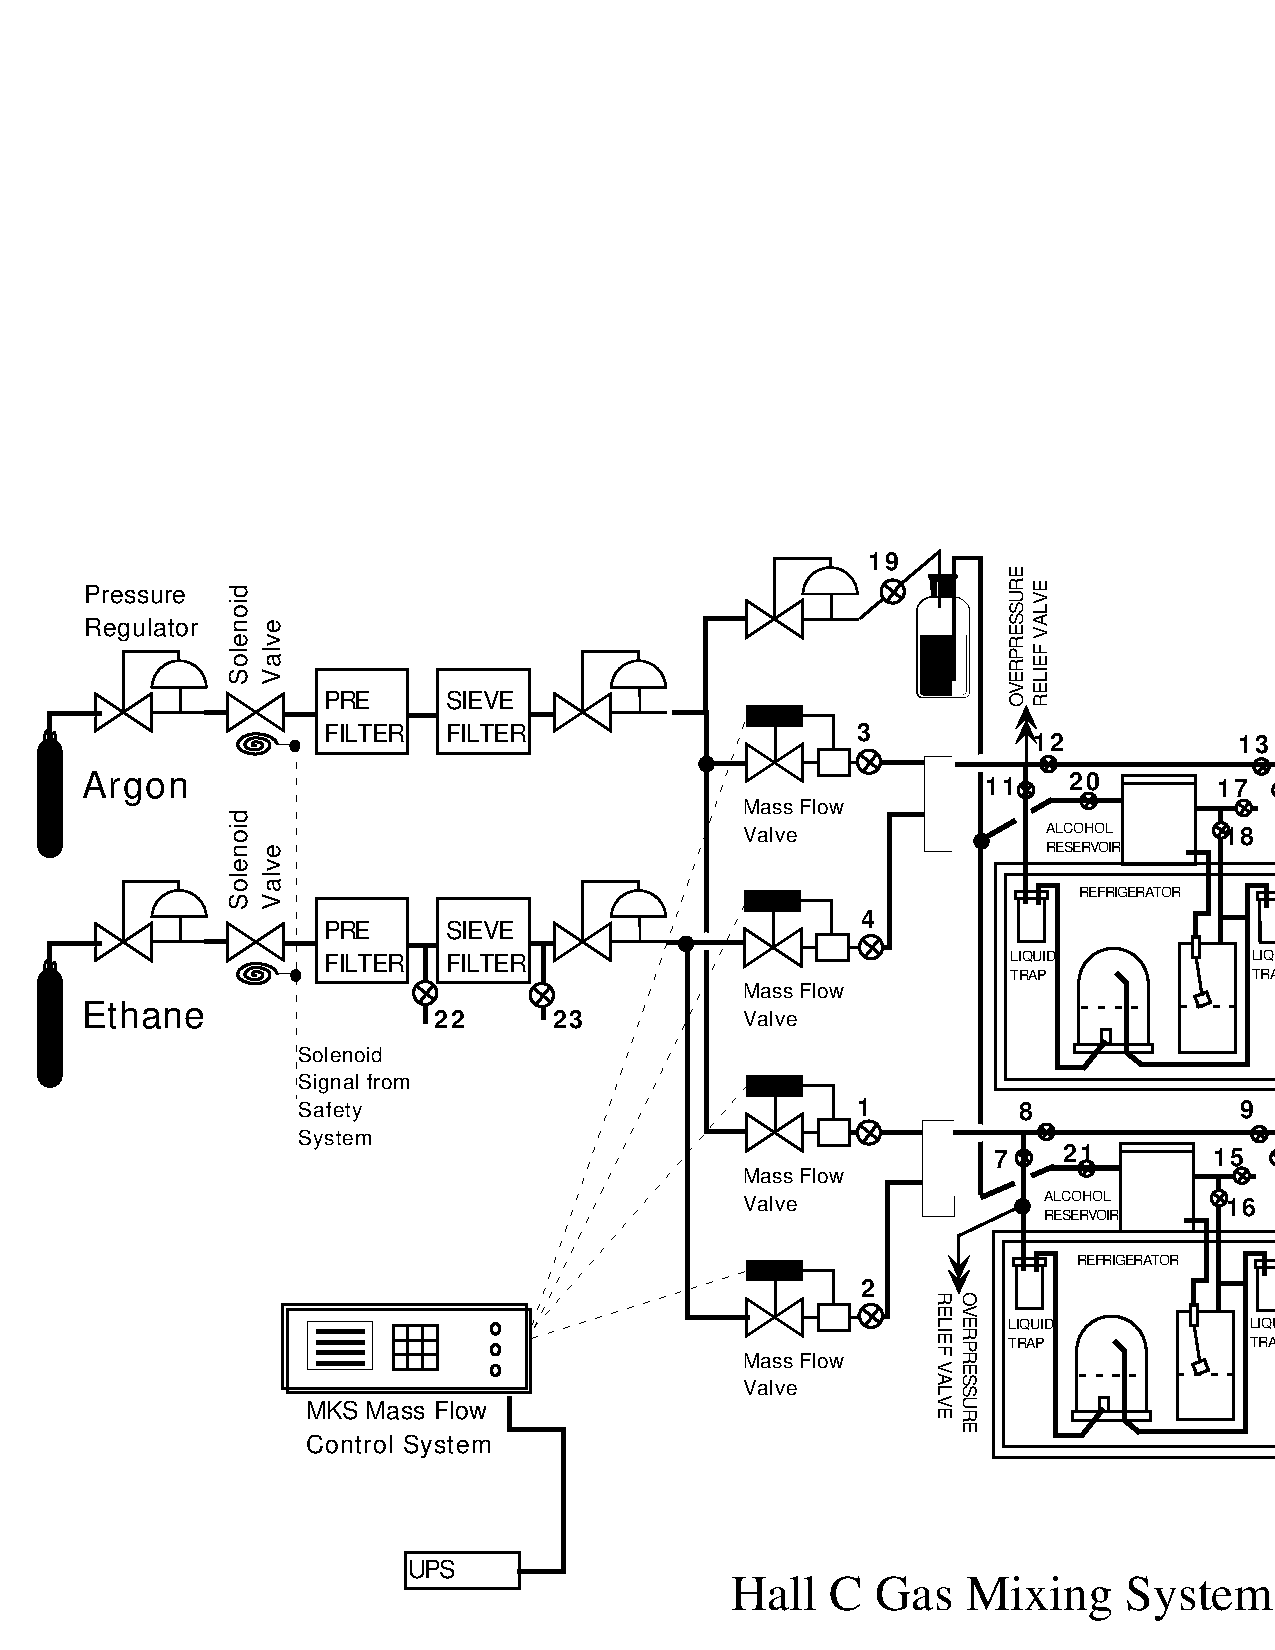
\includegraphics[width=0.9\columnwidth]{HallCGasMixlvl1.pdf}
\caption{Diagram of the Hall~C Gas Mixing System\label{fig:gas_mix}}
\end{figure}

\paragraph{Settings for Normal Operation}

A summary of all of the settings required to make the controller
function properly is given in Table~\ref{tab:mixer_nominals}. The
table also shows which screen contains each parameter. Instructions
for setting parameters are given below. Detailed instructions for
configuring and operating the MKS~647 can be found in the
manufacturer's instruction manual~\cite{647C_EN_0504A1}.

\begin{table}[hbt]
\begin{minipage}[h!]{\textwidth}
{\scriptsize
\begin{center}
\begin{tabular}{|l|c|l|}
\hline
Parameter   & Set To   & {\it Controller Screen}/Comments\\ \hline
\multicolumn{2}{|c|}{\bf Manual Valves  } &  Valves are labeled        \\
Valves 1, 2, 4, 8 & OPEN                  &         \\
Valves 3, 5, 6, 7 & CLOSED                &         \\ \hline
\multicolumn{2}{|c|}{\bf Pressure PID Loop Settings   } & {\it Pressure Control} (Fig. \ref{fig:pressure_control})  \\
Pressure    & 500 Torr &                   \\
PID Mode    & AUTO     &                   \\
PID GAIN    & 4.0      &                   \\
PID INTEG   & 10.0     &                   \\
PID LEAD    & 0.000    &                   \\ \hline
\bf Mixture     & 1        & {\it User} (Fig. \ref{fig:user_display})/ Lower-right corner\\ \hline
\multicolumn{2}{|c|}{\bf Gas Composition for Mixture 1} & {\it Gas Composition} (Fig. \ref{fig:gas_composition})\\
Channel 1   & 1.000    &  (Argon)                 \\
Channel 2   & 1.000    &  (Ethane)                 \\
Channel 3   & 0.000    &                   \\
Channel 4   & 0.000    &                   \\ \hline
\multicolumn{2}{|c|}{\bf MFC Valve Size } & {\it Range Selection} (Fig. \ref{fig:range_selection})  \\
\multicolumn{2}{|c|}{\bf  / Gas}             & {\it Gas Selection} (Fig. \ref{fig:gas_selection})  \\
Channel 1   & 2.0 SLM / Ar         & provides 2.78 SLM Argon\\
Channel 2   & 5.0 SLM / C$_2$H$_6$ & provides 2.50 SLM Ethane\\
Channel 3   & \it unused&                  \\
Channel 4   & \it unused&                  \\ \hline
\multicolumn{2}{|c|}{\bf Channels ON/OFF Settings} & {\it Extended Display} (Fig. \ref{fig:extended_display})   \\
Channel 1   & ON       &                   Press ``ON 1'' (\em Argon)  \\
Channel 2   & ON       &                   Press ``ON 2'' (\em Ethane) \\
Channel 3   & OFF      &                   Press ``OFF 3'' (\em not in use) \\
Channel 4   & OFF      &                   Press ``OFF 4'' (\em not in use) \\ \hline
\multicolumn{2}{|c|}{\bf Pressure Transducer} & {\it Pressure Setup}  \\
Controller  & STD      &                   \\
Range F.S.  & 1000 Torr&                   \\ \hline
\multicolumn{2}{|c|}{\bf MFC Valve Controls     } & {\it Mode Selection} (Fig. \ref{fig:mode_selection}) \\
Channel 1   & PID      &                                   \\
Channel 2   & SLAVE / 1&                                   \\
Channel 3   & INDEP    &                                   \\
Channel 4   & INDEP    &                                   \\ \hline
\bf Alcohol Temp. & 2$^\circ$\,C & Electronic Temperature  \\
                  &              & Control Box             \\ \hline
\hline
\end{tabular}
\end{center}
}%end of \scriptsize
\end{minipage}
\caption{Normal Valve and Parameter Settings for the Gas Mixing System.
\label{tab:mixer_nominals}}
\end{table}
%=====================================================================
\paragraph{General Operation of the Mass Flow Controller}
If the controller screen is dark, press {\bf ESC} to awaken the
display.  Many screens merely provide a menu of other screens you may
access: simply press the item number you desire. To go up one level in
the menu hierarchy, press {\bf ESC}. The \emph{Menu Tree} for the 647C
controller is shown in Fig. \ref{fig:command_tree}.

In general, to change a parameter displayed on the controller screen
use the \textbf{left/ right} arrow keys to move the cursor to the item you
wish to change. Then either use the number keys to enter the value
desired for that item (numeric parameter) or use the {\bf ENTER} or
{\bf up/down} keys to cycle a parameter through its available settings
(configuration parameter). Numeric parameters may be incrementally
modified by using the {\bf up/down} arrow keys. To make certain that a
new parameter becomes active, move the cursor off of the parameter
after you have entered the new value.

The initial menu upon startup is the {\bf Main Menu}
(Fig.~\ref{fig:main_menu}).  For normal operation use the {\bf User
Display} menu (Fig.~\ref{fig:user_display}). It shows the amount of
each gas currently flowing, the total gas flow, and the current
delivery pressure. This display also shows which of several possible
pre-defined gas mixtures is selected. These mixtures are configured
on the {\bf Gas Composition} screen, Fig. \ref{fig:gas_composition}.
For normal operation, we use
only mixture {\bf \#1}, (number shown on the lower-right of the
display). {\bf Only on this screen can this parameter be changed.}
Mixture {\bf \#2} is usually configured to provide 100\% argon for
purging flammable gas out of the chambers.

The {\bf Extended Display} menu (Fig.~\ref{fig:extended_display})
shows actual flow, flow set point, units, valve full-scale range, gas
calibration factor, whether that channel is enabled, and whether each
channel is operating in master, slave, PID, or independent mode. This
display is most useful to a system expert wishing to verify the system
parameter settings.  Most parameters cannot be modified from this
screen, however.

Delivery pressure set-point and pressure \emph{PID-loop} control parameters
may be configured from the {\bf Pressure Control} screen
(Fig.~\ref{fig:pressure_control}).
%
\begin{figure}[tb]
\begin{center}
\framebox{
\begin{minipage}{.65\textwidth}
\footnotesize
\begin{itemize}
\item MAIN MENU (Fig. \ref{fig:main_menu})
   \begin{enumerate}
   \item [1] USER DISPLAY (Fig.\ref{fig:user_display})
   \item [2] EXTENDED DISPLAY (Fig.~\ref{fig:extended_display})
   \item [3] PRESSURE CONTROL (Fig.~\ref{fig:pressure_control})
   \item [4] DIAGNOSTICS
      \begin{enumerate}
      \item [4.1] ERROR LISTING
      \item [4.2] SIGNALS
      \end{enumerate}
   \item [5] INSTRUMENT SETUP
      \begin{enumerate}
      \item [5.1] RANGE SELECTION (Fig.~\ref{fig:range_selection})
      \item [5.2] GAS SELECTION (Fig.~\ref{fig:gas_selection})
      \item [5.3] MODE SELECTION (Fig.~\ref{fig:mode_selection})
      \item [5.4] ZERO ADJUST
      \item [5.5] TRIP LIMITS
      \item [5.6] GAS COMPOSITION (Fig.~\ref{fig:gas_composition})
      \end{enumerate}
   \item [6] SYSTEM SETUP
   \item [7] PRESSURE SETUP
   \item [ ]
   \item [9] INFORMATION
   \item [0] POWER OFF
   \end{enumerate}
\end{itemize}
\end{minipage}
} %%end of \framebox{
\caption{Command Tree for the MKS-647C Control Panel}
\label{fig:command_tree}
\end{center}
\end{figure}
%
\begin{center}
\begin{figure}[hbt]
\begin{minipage}{2.7in}
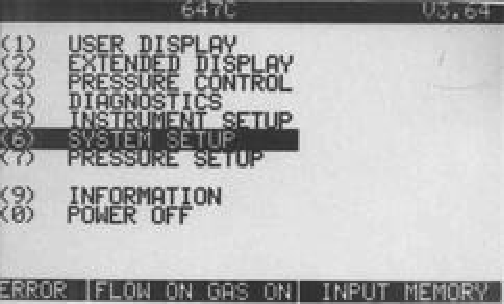
\includegraphics[width=2.6in,height=1.8in]{drift_gas_system-main_menu-eps-converted-to.pdf}
\caption{MKS~647 Main Menu\label{fig:main_menu}}
\end{minipage}
\begin{minipage}{2.7in}
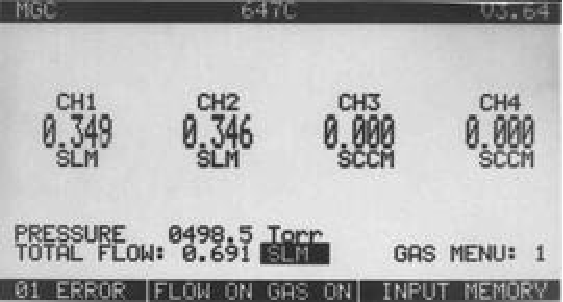
\includegraphics[width=2.6in,height=1.8in]{drift_gas_system-user_display-eps-converted-to.pdf}
\caption{MKS~647 User Display\label{fig:user_display}}
\end{minipage}
\end{figure}
\end{center}
%
\begin{center}
\begin{figure}[hbt]
\begin{minipage}{2.7in}
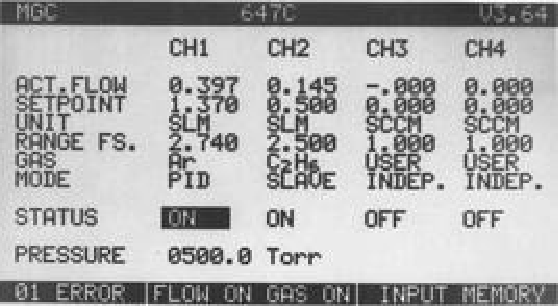
\includegraphics[width=2.6in,height=1.8in]{drift_gas_system-extended_display-eps-converted-to.pdf}
\caption{Extended Display Screen\label{fig:extended_display}}
\end{minipage}
\begin{minipage}{2.7in}
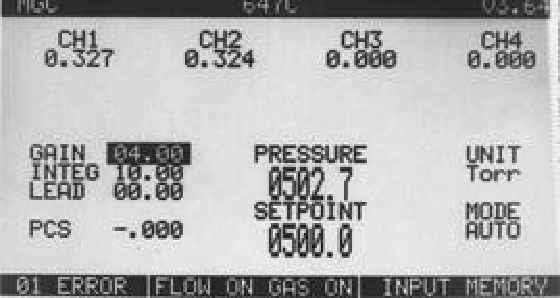
\includegraphics[width=2.6in,height=1.8in]{drift_gas_system-pressure_control-eps-converted-to.pdf}
\caption{Pressure Control Screen\label{fig:pressure_control}}
\end{minipage}
\end{figure}
\end{center}
%=====================================================================
\paragraph{Gas Flow Rates}
\label{sec:gas_flow_rates}
The flow rates are adjusted automatically by the controller in order
to maintain a constant delivery pressure at the output. Only the flow
{\em ratios} should be set by the operator. We use a 1:1 ratio, set on
the {\bf Gas Composition} screen (Fig.~\ref{fig:gas_composition}), as
indicated in Table~\ref{tab:mixer_nominals}.

The average total flow should equal the sum of the flows to all of the
detectors in the shield house. (Note that the ball-type flowmeters in
the shield house are calibrated for nitrogen. The approximate
multiplier to convert these readings for 50/50 Argon-Ethane is 0.9 .)

System configuration parameters specifying the full-scale flow
capacity (for nitrogen) of each valve, the types of gases actually
flowing through each valve, and the mode of control for the valves are
set in the screens pictured in Figs.~\ref{fig:range_selection},
\ref{fig:gas_selection}, and \ref{fig:mode_selection}. These figures
show the nominal settings for the Hall-C system.

\begin{center}
\begin{figure}[hbt]
\begin{minipage}{2.7in}
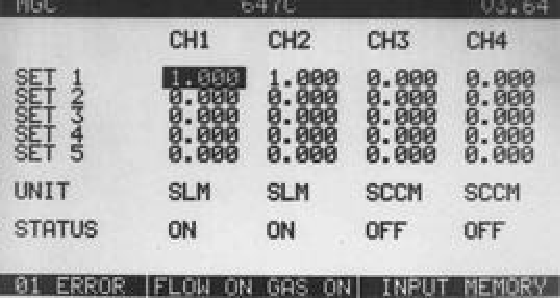
\includegraphics[width=2.6in,height=1.8in]{drift_gas_system-gas_composition-eps-converted-to.pdf}
\caption{Gas Composition Screen\label{fig:gas_composition}}
\end{minipage}
\begin{minipage}{2.7in}
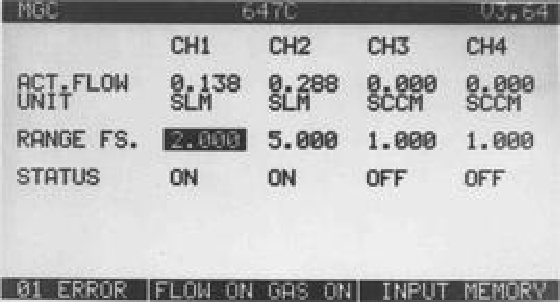
\includegraphics[width=2.6in,height=1.8in]{drift_gas_system-range_selection-eps-converted-to.pdf}
\caption{Range Selection Screen\label{fig:range_selection}}
\end{minipage}
\end{figure}
\begin{figure}[hbt]
\begin{minipage}{2.7in}
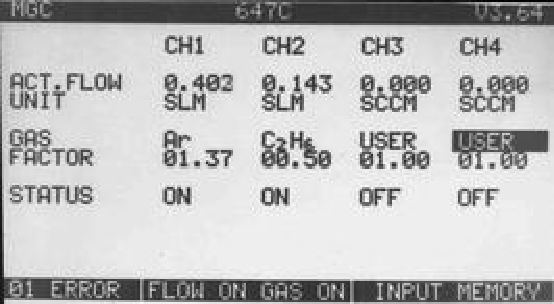
\includegraphics[width=2.6in,height=1.8in]{drift_gas_system-gas_selection-eps-converted-to.pdf}
\caption{Gas Selection Screen\label{fig:gas_selection}}
\end{minipage}
\begin{minipage}{2.7in}
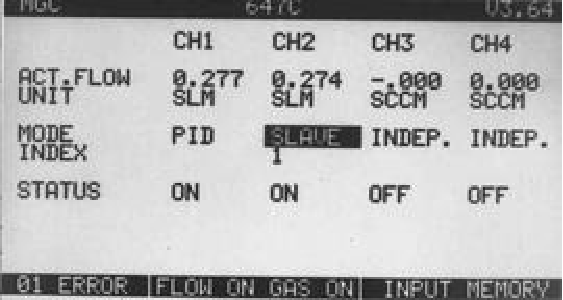
\includegraphics[width=2.6in,height=1.8in]{drift_gas_system-mode_selection-eps-converted-to.pdf}
\caption{Mode Selection Screen\label{fig:mode_selection}}
\end{minipage}
\end{figure}
\end{center}

%=====================================================================
\paragraph{To set the Delivery Pressure:}

Navigate to the {\bf Pressure Control} menu. The pressure set-point (in
Torr) is indicated at the bottom-center of the screen. This value
should be set to 500.0. Note that the system can not respond instantly
to a change in requested gas pressure: it has no way to release excess
pressure and must wait for the detector systems to consume it
\footnote{An \emph{over-pressure relief valve} releases gas through a
small oil bubbler in the gas shed if the pressure exceeds about
600~Torr.}; it cannot build up pressure any faster than the
flow-control valves can supply it. It may take thirty minutes or so
for the pressure regulation system to stabilize at a new set-point or
stabilize in response to a change in total gas consumption. However,
you should be able to observe a change in the gas flow within a few
seconds (possibly up to a minute) after a set-point change.

%=====================================================================
\paragraph{To turn gas flow on or off:}

The gas flow can be turned on or off while in any menu.  In the
Extended Display menu the bottom line displays ``ON'' or ``OFF'', by
channel, to show which mass flow valves are enabled.  ``ON'' must be
displayed in the bottom row of the Extended Display menu for gas to be
flowing in a particular channel.

For gas to flow, two conditions must be met:
\begin{enumerate}
\item Each channel (1 and 2) must be enabled by pressing ``ON'' and then the
  desired channel number.
\item The entire system must be enabled by pressing ``ON" and then ``ALL" from
  the keypad.
\end{enumerate}
Thus, each valve can be controlled individually using ``ON/OFF~-~\emph{Channel
Number}'', or all flow can be controlled using ``ON/OFF~-~ALL''. If the system
is enabled, the status line at the bottom of every screen will indicate ``FLOW
ON GAS ON''. {\bf Note:} because Valve-2 (ethane) is normally slaved to Valve-1
(argon), when Valve-1 is disabled there will be no flow through Valve-2.

%=====================================================================
\paragraph{To Change a Gas Bottle}

Only authorized personnel are permitted to change gas bottles.

The argon and ethane supply bottles should be replaced by new (full)
bottles when the bottle content drops below about 10\% of its
capacity.  For argon, the bottle content is directly indicated by the
bottle pressure: a new bottle usually contains 2000 to
3000~psig. Argon bottles should be changed whenever the bottle
pressure is found to be below about 200~psig.

Ethane bottles, on the
other hand, contain liquefied ethane. Thus the bottle pressure is just
the vapor pressure of ethane at whatever the current temperature
happens to be. At 70$^\circ$\,F this is about 544~psig. The pressure gauge
will not tell you how much ethane is left in the bottle until it reads
zero! Instead, we measure the ethane content by observing the weight
of the bottle and comparing it to the weight when the bottle was
full. A standard B-size cylinder contains about 32~pounds of ethane.
The ethane cylinders on the manifold sit on scales which have been
pre-set to indicate the net weight of ethane in the bottle.
Numbers in the green portion of the dial indicate ethane remaining.
If the indicator points to the red portion of the dial, the bottle
is empty.

Handling and connecting bottles of compressed gas require special
knowledge.  The high pressure gas stored in the cylinders (bottles)
constitutes significant stored energy. Mishandling of a gas bottle can
pose a lethal hazard! Refer to the JLab ESH\&Q Manual
for safe handling practices. If you do not already know how to safely
manipulate compressed gas hardware, have a knowledgeable person train
you.

After attaching a new gas bottle to the supply manifold, check the
connection for leaks using \emph{Snoop} or a similar leak detector.

%=====================================================================
\paragraph{The Alcohol Bubbler}

To reduce the rate of aging of the wire chambers, the operating gas
contains a small quantity of alcohol vapor. The vapor is added by
bubbling the argon/ethane mixture through liquid alcohol. The
temperature of the alcohol controls the alcohol vapor pressure, which
determines the amount of vapor added to the gas. The alcohol content
also affects the electron drift velocity in the wire chambers, so it
must be held approximately constant.

Gas is bubbled through the liquid alcohol inside the glass
dome vessel in the refrigerator. The dome is covered by a
perforated steel cylinder as a precaution against breakage. The
alcohol level is controlled by a float valve inside the metal cold
reservoir, which is also inside the refrigerator. As long as there is
alcohol in the warm reservoir (sitting on top of the refrigerator),
the liquid levels inside the refrigerator will remain constant. A
drain valve (\#7) inside the refrigerator is available for emptying
all liquid from the system.  It is for use by experts only and should
remain closed during normal operation.

%=====================================================================
\subparagraph {Alcohol Temperature Control}

To keep the alcohol temperature (and thus the vapor pressure) constant,
the alcohol bubbler is housed in a refrigerator which is controlled by
an electronic temperature regulator having 1$^\circ$C sensitivity. The
controller is located on a shelf in the right-hand rack of the gas mixing
system. Normally, the actual temperature in the refrigerator is
indicated on the front panel of the controller. The controller should
be set to maintain a temperature of 2$^\circ$\,C.

%=====================================================================
}
\begin{safetyen}{0}{0}
\infolevone{\subsubsection{Safety Information}}
\label{sec:hallc-det-gasalarms}

\infoleveqnull{\subsection{Hazards}}
\infolevone{\paragraph{Hazards}}

Some of the gases that are used are flammable.  Also, the gas bottles
are under high pressure and can become missiles.

\infoleveqnull{\subsection{Mitigations}}
\infolevone{\paragraph{Mitigations}}

The bottles are located in a fenced area next to the gas shed with the bottles
secured so that they can not fall.

In the Hall C counting house, alarms for the gas system
are integrated into the VESDA system located on the left side
of the control console.  The VESDA system will go into
alarm if elevated levels of flammable gas are present in
either of the two spectrometer detector huts or the gas shed.
Response to an alarm should be to contact the personnel listed below.

\infoleveqnull{\subsection{Responsible Personnel}}
\infolevone{\paragraph{Responsible Personnel}}

Maintenance of the gas systems is routinely performed by the Hall c
technical staff.  Shift personnel are not expected to be responsible
for maintaining the detector gas systems (see Table \ref{tab:gas:personnel}
for the names of persons to be contacted in case of problems).

\begin{namestab}{tab:gas:personnel}{Gas for wire chambers: authorized personnel
}{%
      Responsible personnel for detector gas system.}
  \TechonCall{\em Contact}
  \LarryCarraway{}
  \JerryNines{}
  \JoeBeaufait{}
  \BradSawatzky{}
  \JackSegal{}
  \MahlonLong{}
\end{namestab}
\end{safetyen}
